\documentclass[UTF8,a4paper,12pt]{ctexart}
\usepackage{algorithm} %format of the algorithm 
\usepackage{algorithmic} %format of the algorithm 
\renewcommand{\algorithmicrequire}{ \textbf{Input:}}     %Use Input in the format of Algorithm
\renewcommand{\algorithmicensure}{ \textbf{Output:}}    %UseOutput in the format of Algorithm
\usepackage{multirow} %multirow for format of table 
\usepackage{amsmath} 
\usepackage{xcolor}
\usepackage{booktabs}%加载 booktabs 宏包之后可以使用 \toprule 和 \bottomrule 命令分别画出表格头和表格底的粗横线,而用 \midrule 画出表格中的横线
\usepackage{diagbox} %加载 diagbox 宏包之后可以绘制斜线表头
\usepackage{multirow} %加载 multirow 宏包后可以让表格单元实现合并与分割
\usepackage{makecell} %加载 makecell 宏包可以在表项中使用"\\"命令自由的换行。在不打算固定表列宽度时,它比p{宽度}选项更为灵活。
\usepackage{longtable} %加载 longtable 宏包可以处理行数非常多的长表格
\usepackage{array}
\usepackage{tabularx}
\usepackage{ctex}
\setcounter{secnumdepth}{4}
\setcounter{tocdepth}{4}
\usepackage{amsmath}
\numberwithin{equation}{section}
\allowdisplaybreaks[4]       %多行公式中换页
\usepackage{array}
\usepackage[font=small,font=bf,labelsep=none]{caption}
\usepackage{amssymb}
\usepackage{tikz}
\usepackage{amsthm}
\usepackage{mathrsfs}
\usepackage{dutchcal}
\usepackage{color}
\usepackage{graphicx}    %插入图片
\usepackage{times}
\usepackage{mathptmx}
\usepackage{fancyhdr} %页眉页脚
\pagestyle{fancy}
\fancyhf{}
\fancyfoot[C]{\thepage}
\usepackage{setspace}
\setlength{\baselineskip}{20pt}
\newcommand*{\circled}[1]{\lower.7ex\hbox{\tikz\draw (0pt, 0pt)%
    circle (.5em) node {\makebox[1em][c]{\small #1}};}}
\usepackage{hyperref}  %目录
\hypersetup{colorlinks=true,linkcolor=black}
\renewcommand {\thefigure} {\thesection{}-\arabic{figure}}%设定图片的编号。这样设置的实现效果为图1-1
\renewcommand {\thetable} {\thesection{}-\arabic{figure}}
\usepackage{caption}
\captionsetup{font={small},labelsep=quad}%文字5号,之间空一个汉字符位。
\captionsetup[table]{font={bf}} %表格表号与表题加粗
\usepackage{appendix}
\usepackage{tocloft} 
\renewcommand{\cftsecleader}{\cftdotfill{\cftdotsep}} %为目录中section补上引导点
\usepackage{titletoc}
\titlecontents{section}[0pt]{\addvspace{6pt}\filright\bf}%
               {\contentspush{\thecontentslabel \quad}}%
               {}{\titlerule*[8pt]{.}\contentspage}
\makeatletter %双线页眉
\def\headrule{{\if@fancyplain\let\headrulewidth\plainheadrulewidth\fi%
\hrule\@height 1.5pt \@width\headwidth\vskip1.5pt%上面线为1pt粗
\hrule\@height 0.5pt\@width\headwidth  %下面0.5pt粗
\vskip-2\headrulewidth\vskip-1pt}      %两条线的距离1pt
  \vspace{6mm}}     %双线与下面正文之间的垂直间距
\makeatother
\CTEXsetup[format={\heiti \zihao{3} \bfseries \center}]{section}
\CTEXsetup[number={第\chinese{section}章}]{section} 
\usepackage[explicit]{titlesec}
\titlespacing*{\section}{0pt}{24pt plus .24pt minus .24pt}{18pt plus .0ex}

\begin{document}

\thispagestyle{empty}

\renewcommand{\headrulewidth}{0pt}
\begin{figure}[htb] 
 \center{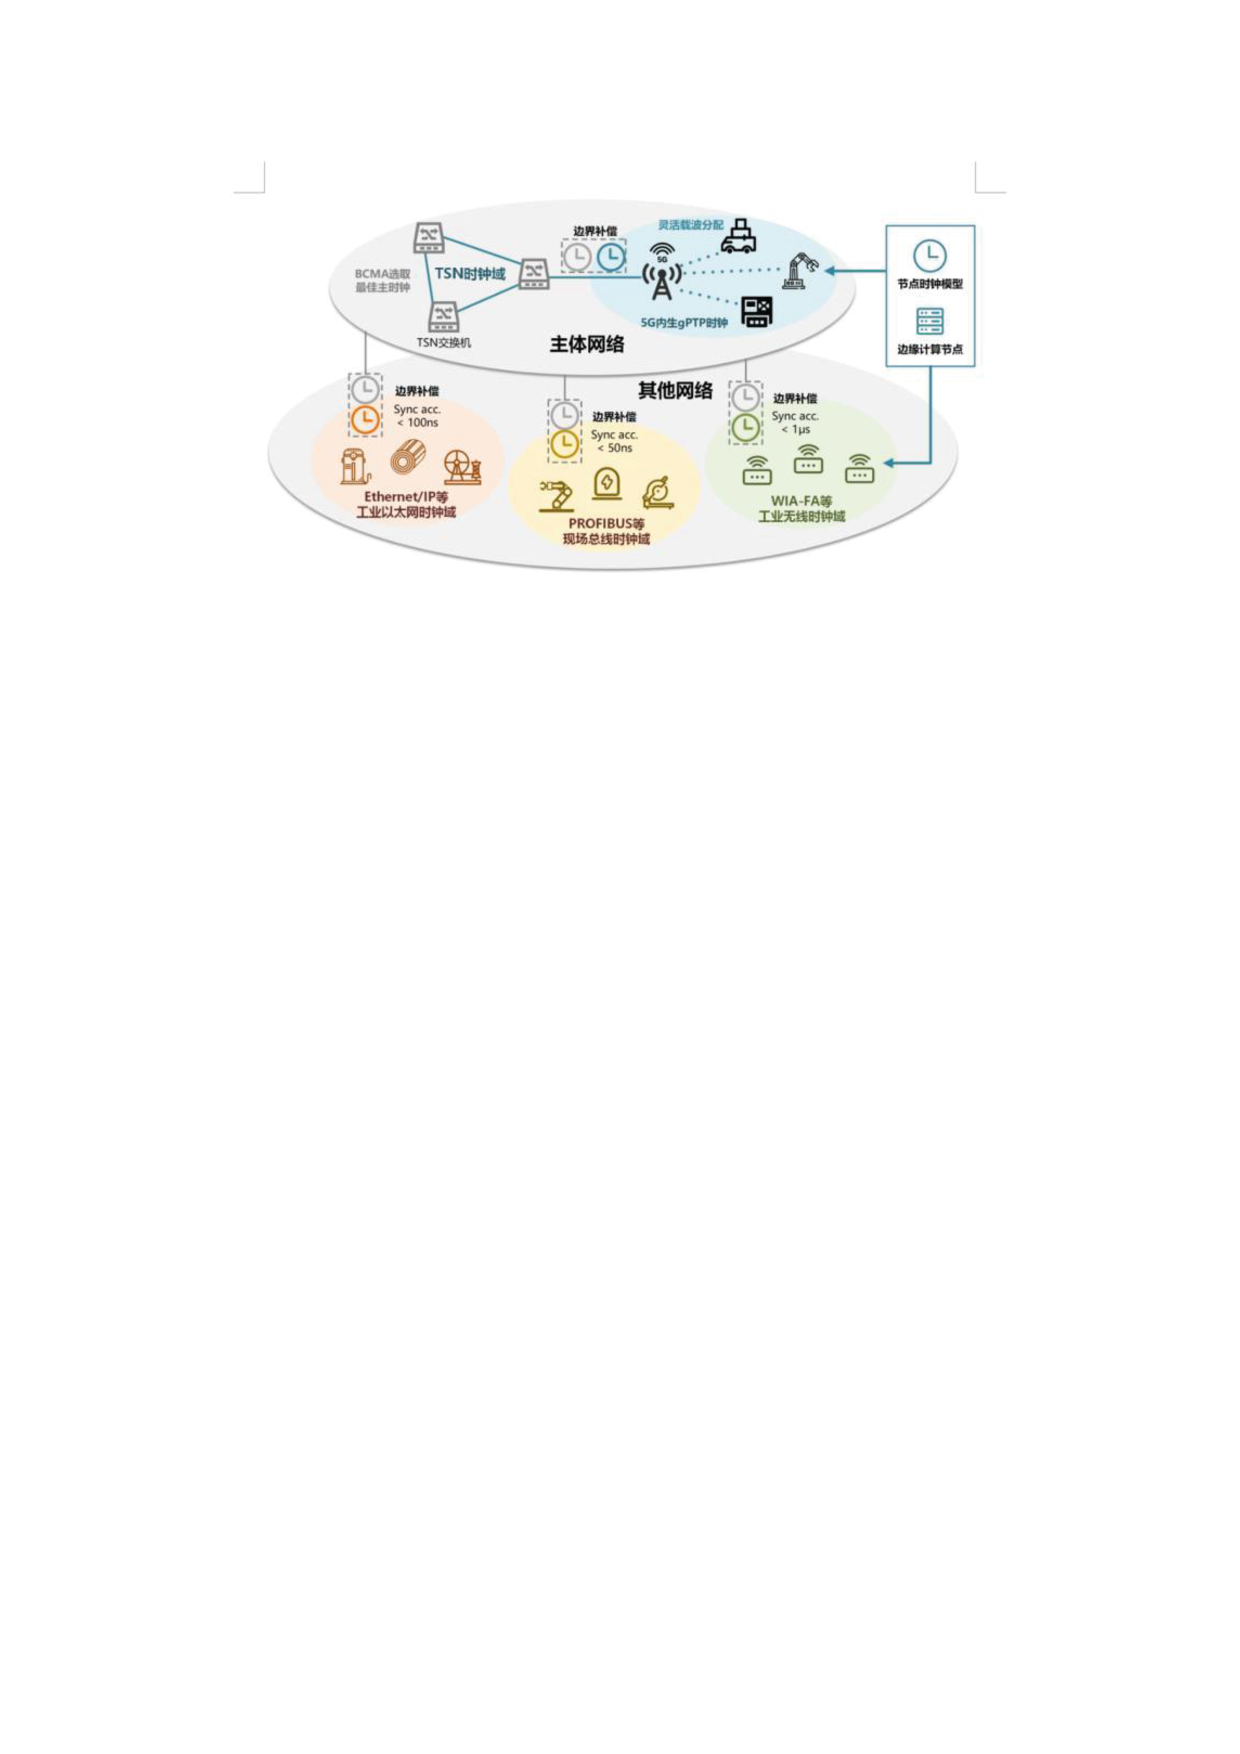
\includegraphics[width=5cm]  {fig1.png}} 
 \end{figure}

\begin{center}
\songti \zihao{-2} 上海交通大学学位论文
\end{center}
%该页为中文扉页。无需页眉页脚,纸质论文应装订在右侧
~\\
\begin{center}
\songti \zihao{1} \textbf{上海交通大学学位论文格式模板}
\end{center}
%中文论文标题,1行或2行,宋体,加粗,二号,居中。论文题目不得超过36个汉字
~\\
~\\
~\\
~\\
\begin{center}
\heiti \zihao{4}
\begin{tabular}{l}
\textbf{姓\quad名:陈相}\\
\textbf{学\quad号:119032910097}\\
\textbf{导\quad师:陈彩莲}\\
\textbf{学\quad院: 电子信息与电气工程学院}\\
\textbf{学科/专业名称:控制工程}\\
\textbf{申请学位层次:硕士学位}\\
\end{tabular}
\end{center}
~\\
\begin{center}
\songti \zihao{4} \textbf{20XX年XX月}
\end{center}

\newpage
\thispagestyle{empty}
~\\
\begin{center}
\zihao{4}
\textbf{
A Dissertation Submitted to \\
Shanghai Jiao Tong University for Master/Doctoral Degree}
\end{center}
~\\
\begin{center}
\zihao{-2}\textbf{
DISSERTATION TEMPLATE FOR MASTER DEGREE OF ENGINEERING IN \\
SHANGHAI JIAO TONG UNIVERSITY}
\end{center}
%英文论文标题:大写,Times New Roman,加粗,14 points,居中
~\\
~\\
~\\
\begin{center}
\zihao{3} 
Author:  \\
Supervisor:  
\end{center}
~\\
~\\
~\\
\begin{center}
\zihao{3} 
School of XXXXXXX \\
Shanghai Jiao Tong University \\
Shanghai, P.R.China \\
June 28th, 2021  
\end{center}

\newpage
\thispagestyle{empty}
\begin{center}
\heiti \zihao{3}\textbf{
上海交通大学\\
学位论文原创性声明}
\end{center}

\zihao{-4}
本人郑重声明:所呈交的学位论文,是本人在导师的指导下,独立进行研究工作所取得的成果。除文中已经注明引用的内容外,本论文不包含任何其他个人或集体已经发表或撰写过的作品成果。对本文的研究做出重要贡献的个人和集体,均已在文中以明确方式标明。本人完全知晓本声明的法律后果由本人承担。

\begin{flushright}
\begin{tabular}{l}
\zihao{4}
学位论文作者签名:\hspace{20mm}\qquad\\
\zihao{4}
日期:\qquad年\qquad月\qquad日
\end{tabular}
\end{flushright}

~\\
\begin{center}
\heiti \zihao{3}\textbf{
上海交通大学\\
学位论文使用授权书}
\end{center}

本人同意学校保留并向国家有关部门或机构送交论文的复印件和电子版,允许论文被查阅和借阅。\\
本学位论文属于 :\par
□公开论文\par
□内部论文,保密□1年/□2年/□3年,过保密期后适用本授权书。\par
□秘密论文,保密\_\_\_年(不超过10年),过保密期后适用本授权书。\par
□机密论文,保密\_\_\_年(不超过20年),过保密期后适用本授权书。\par
(请在以上方框内选择打“√”)\\

\begin{flushright}
\zihao{4}
\begin{tabular}{l l}
学位论文作者签名:\hspace{10mm}\qquad \hspace{100mm}&指导教师签名:\qquad\\
日期:\qquad年\qquad月\qquad日 &日期:\qquad年\qquad月\qquad日\\
\end{tabular}
\end{flushright}

\newpage
\pagenumbering{Roman}
\fancyhead[LH]{上海交通大学学位论文}
\fancyhead[RH]{第一章\quad绪论}

\addcontentsline{toc}{section}{摘\quad要}
\section*{摘\quad要}
%摘要:二字间空一格,黑体16磅加粗居中,单倍行距,段前24磅,段后18磅。

\hspace{8mm}学位论文是研究生从事科研工作的成果的主要表现,集中表明了作者在研究工作中获得的新的发明、理论或见解,是研究生申请硕士或博士学位的重要依据,也是科研领域中的重要文献资料和社会的宝贵财富。\par 
为了提高研究生学位论文的质量,做到学位论文在内容和格式上的规范化与统一化,特制作本模板。\\
~\\
\textbf{关键词}:学位论文,论文格式,规范化,模板\\
%关键字:宋体12磅,行距20磅,段前段后0磅,关键字之间用逗号隔开,关键词三个字加粗。

\newpage
\addcontentsline{toc}{section}{ABSTRACT}
\section*{ABSTRACT}
%ABSTRCT:Arial 16磅加粗居中,单倍行距,段前24磅,段后18磅

\hspace{8mm}As a primary means of demonstrating research findings for postgraduate students, dissertation is a systematic and standardized record of the new inventions, theories or insights obtained by the author in the research work. It can not only function as an important reference when students pursue further studies, but also contribute to scientific research and social development.\par 
This template is therefore made to improve the quality of postgraduates’ dissertation and to further standardize it both in content and in format.\\
%英文摘要内容:Times New Roman 12磅,行距20磅段前段后0磅
~\\ 
\textbf{Key words}: dissertation, dissertation format, standardization, template
%Keywords:Times New Roman 12磅,行距20磅, “key words” 两词加粗

\newpage
\renewcommand\contentsname{\textbf{目\quad录}}
\begin{center}
{\tableofcontents
\thispagestyle{fancy}
\fancyhead [RO, LE] {\normalsize{\songti 第一章\quad绪论}}
\fancyhead [LO, RE] {\normalsize{\songti 上海交通大学学位论文}}
}
\end{center}

\newpage
\pagenumbering{arabic}
\section{绪论}
\subsection{研究背景}
近年来,诸如工业自动化,IoT(Internet of Things)之类的技术增长了许多倍,应用变得至关重要。[1]云计算和高速网络的兴起要求高度精确的时间同步[2]。廉价的振荡器或石英晶体的特性会随功率,老化和热量的变化而变化。因此,不能保证两个相似的晶体以相同的时间/频率振荡。这些限制使振荡器的运行与其他振荡器略有不同。对于大型基础架构而言,用昂贵的时钟代替计算机的内置廉价时钟是不可行的。因此,一种有力而有效的方式来同步已传播结构的时钟是必不可少的[3]。NTP(Network Time Protocol)是时钟同步的最广泛使用的解决方案。后来,一种更精确的解决方案称为PTP,已被证明对时钟同步更有利[4]。尽管PTP通信算法与NTP类似,但PTP在事件的精确硬件辅助时间记录上却有所不同,称为时间戳[5]。 PTP是可以实现高精度时钟同步的一种可行解决方案。时钟同步是工业网络中非常重要的一环,而且对于时钟同步的要求也是越来越高的,其中无线和有线的时钟同步精度也是有着较大的差别。在有线领域,早期NTP的时钟同步精度由于是协议层的时间戳,误差一般达到10μs以上,再后来1588的时钟同步利用硬件时间戳,将精度提到到了几十纳秒到几十亚微秒间,同时减少了时钟同步对外部GPS信号的依赖,现在TSN(Time Sensitive Network)的802.1AS使用1588的同步方案,同时完全使用mac层的信息交互,减少了各层级之间的延迟误差,将同步精度稳定在了纳秒级,在具体的工业网络场景中,例如在现有的工业控制网络ethercat中,利用“分布时钟”机制,可以实现小于1μs的时钟同步精度。[6]在无线领域,时钟同步由于无线情况下的能量约束,本身报文时间粒度不高,传输过程中的干扰,本身同步精度要求不高等问题,精度一直停留在微秒级别。但是在5G的应用场景例如载波聚合,多点协同中,同步精度则要求达到100ns级别[7]。


TSN由于其高确定性网络而由于成为当前热门,TSN作为时间敏感网络,拥有诸如Qbv等门控调度算法保护来保证时间敏感流的传输,现在做调度算法的有很多,但有一个假设前提:时钟同步是完美的,不存在同步误差和误差抖动;但是,在实际工业场景中假设不成立。TSN对于时钟同步的精度要求极高(ns级别),目前的TSN的同步协议802.1AS,在可接受的误差范围内,有线网络可以提供高精度的时钟同步,但是当网络规模较大,跳数增多,背景流量增多时,同步精度会大幅下降,从而影响整个TSN的性能。[8]换言之,TSN本身收到有线网络的局限性,需要通过与无线异构来解决有线跳数过多的问题,且在工厂内部的复杂环境下,本身就可能存在的多种无线设备与有线设备异构的情况,仅仅通过保证TSN有线网络内部的高精度同步无法满足实际的应用场景。为将TSN和无线网络相互结合,需要进一步考虑异构网络下的时钟同步方法,可以通过双层网络架构来降低网络规模对于整个同步精度的影响,也就是TSN+无线解决方案,即上层GM(Grand Master)到基站采用有线TSN结构,下层采用无线网络来同步从节点,这种情况下,无线网络的高覆盖性,可以有效降低网络规模较大的情况下跳数对于同步精度的影响,为TSN提供了一个更加有实际意义的应用场景。


针对这种有线无线网络异构结构,这些年也有很多时钟同步方案被提出,用来解决异构网络的协同问题,不同的同步方法有着其适用的范围,而对于大规模无线网络节点的异构同步方案,目前没有比较好的同步解决方案。

\subsection{研究现状}
为解决异构网络的同步问题,通常都会选择选择先优化有线网络同步精度,将其作为主时钟后再针对无线网络进行主从同步。
有线网络部分的时钟同步,目前精度最高的有线网络同步为时间敏感网络的同步方案,时间敏感网络(Time Sensitive Network),简称TSN,采用TSN中协议802.1AS规定的时钟同步方案,此此方案是根据1588时钟同步方案改进而来,采用主从式同步方法,主从节点之间通过交换时间戳进行上下行延迟进行测量,得到两节点之间的传输延迟,进一步得到时钟偏差。事实上,两节点之间的传输延迟由报文传播延迟,高斯噪声,不确定性延迟组成,后两者是造成时钟同步精度误差的主要原因。在有线网络中,由于较高的稳定性和较好的传输性能,这两部分一般选择忽略不计,即将上下行传输延迟作为对称延迟来进行处理。[8]


相比于有线情况的时钟同步,无线网络中的能量约束,以及节点之间的传输干扰,造成无线时钟同步的误差较大。高精度的无线时钟同步的研究目前主要针对WSN和5G。

如果是倾向于高精度的无线时钟同步方案,在同步方法上,更多是采用类似1588的上下报文测量传输延迟的同步方案,在网络结构上,更多是采用类似于聚类的网络结构。聚类网络结构时钟同步的出发角度有从能量的角度出发进行考虑的,也有单纯从精度的角度出发进行考虑的。精度的方面,Xiangli Jia和Yang Lu针对网络跳数对于同步精度的影响做了专门的分析,得出了聚类网络结构相对于传统多跳网络结构的优势[9]。Jie Wu,Liyi Zhang则在聚类网络的结构基础上,提出了通过计算共识时钟来进行同步的方案。从能量的角度出发进行考虑的聚类网络结构,更多是从聚类算法的角度进行研究[10]。Pengyi Jia提出通过时钟频率抖动的大小s来进行网络聚类,通过将性能较差的时钟节点聚类进行同步的方式,可以有效降低网络整体的时钟同步频,从而达到降低网络整体能耗的目的[11]。Parminder Kaur也在文章中提出可以通过就近原则的聚类方法,来降低所有节点间通信距离差的和,来达到降低能耗的目的[12]。


针对传统的WSN网络中的聚类时钟同步在现实的应用问题,文献 [13] 等人研究了这些聚类结构时钟同步在5G中的可行性,并提出了可能存在的挑战以及可能的解决方案。5G下的时钟同步,主要是通过BS来完成上层与下层网络之间的同步。但是目前用来传输时间信息的报文SIB16时间精度不高,这就造成了影响时间同步精度关键的时间戳精度不高,而且无线时钟同步方案的时间戳采用的是应用层的时间戳,应用层时间戳在产生过程中很可能会产生较大的非确定性延迟,例如排队延迟,这类延迟通常数量级较大,在传统时钟同步方案中由于产生概率较低,通常放弃对这部分延迟的建模,但是当网络规模增大时,这类延迟的产生概率也会随着增加,从而对时钟同步精度产生较大的影响。如果要实现像TSN的802.1AS一样的高精度时间同步,必须对这一类延迟进行建模补偿,从而才能使得无线网络和有线TSN时钟同步实现对接。 


在很多研究中,无线网络只是作为一个性能较差的有线网络来进行建模,所谓的异构网络,仅仅只是两个性能不同的有线网络连接在一起,然而事实上,根据文献[14],[15]所述,无线网络和有线网络对接的过程中,之所以会产生较大的同步误差,很大原因是由于在上行回传的过程中,会产生较大的PDV(packet delay variation),从而严重影响同步性能。众所周知,定时数据包中的PDV(即延迟抖动)是降低IEEE 1588系统中同步精度的主要因素。 PDV是由于交换集线器上的数据包排队而产生的。 例如,在具有快速以太网接口的交换集线器中,如果在时序数据包到达时仅一个最大传输单元(MTU)大小为1518字节的数据包位于缓冲区中,则排队延迟最多变化122.4μs。这显然会较大地影响同步性能,造成有线网络和无线网络部分的对接困难。即不能很好地实现5G和有线TSN的对接。
为了克服由于延迟抖动引起的同步性能的下降,已经广泛研究了各种同步过程。文献[16],[17]具有以太滤波方法或统计方法的反馈回路是一种基本机制。但是,反馈系数是根据经验确定的。因此,通常很难自适应地优化它们。因此,就稳定性和准确性而言,可能难以获得足够的同步性能。


文献[18],[19]为了减轻由于延迟抖动引起的同步精度下降,提出了一种使用探测数据包进行排队估计的方法。采用探测数据包的目的是估计定时数据包中延迟抖动的发生,并且 过滤出具有时延抖动的数据包。这种方法可以有效测出当前的实际网络排队延迟大小,但是过程过于繁琐,且容易造成新增流量过多,能耗增大的问题。


文献[20],[21]指出诸如IEEE 1588精确时间协议和网络时间协议之类的时序协议要求对时间服务器(主服务器)与客户端(从属服务器)之间的通信路径延迟进行精确测量,以提供精确的时序同步。然后,使用这样的假设来估计客户站点上的准确时间,该假设是由于通过网络的物理传播时间引起的前向和后向延迟相等,或者它们之间的任何差异都是预先校准的。除了物理链路延迟之外,由于路径上的交换/路由设备,定时数据包还会遇到队列引起的延迟。将排队延迟归于非对称延迟中,并针对齐设计了补偿算法。但是其补偿算法依然依赖每次测量得到的数据,对于时钟同步来说过于繁琐。


文献[22]指出基于经典双向消息交换方案的IEEE 1588是用于分组交换网络的流行时钟同步协议。由于数据包交换网络中存在随机排队延迟,因此时钟偏斜和与已交换同步数据包时间戳之间的偏移的联合恢复可以视为统计估计问题。在前向主从路径与反向从主路径的确定性路径延迟之间可能存在未知性的情况下,IEEE 1588的时钟偏斜和偏移估计问题来自不正确的建模或网络攻击。首先,假设多个主从通信路径的可用性以及对描述随机排队延迟的概率密度函数的全面了解,该文章针对IEEE 1588的时钟偏斜和偏移估计方案,针对均方估计误差开发了下限。通过混合高斯随机变量来近似随机排队延迟的概率密度函数,该文章提出了一种鲁棒的迭代时钟偏斜和偏移估计方案,该方案采用空间交替广义期望最大化(SAGE)算法来学习所有未知参数。数值结果表明,所开发的鲁棒方案显示出接近下限的均方估计误差。这篇文章通过引入高斯混合分布来对排队延迟建模来达到了更好的时钟偏差估计,但整个计算过程过于复杂,传输开销较大。


实际应用过程中,由于5G网络低延迟,高精度的特性,是最有可能成为未来无线TSN载体的通信协议。目前针对5G和TSN融合的问题,3GPP协议和各通信厂商给出的解决方案为5G网桥。通过CNC对5G网络分配网桥的角色,并在有线无线交接处的协议转换器记录时间戳来计算5G网络内部的驻留时间,从而实现5G网络两端的TSN有线设备满足同步要求。但是该方案并不能满足未来无线TSN设备的同步需求,因为其并没有解决无线网络内部的累积同步误差问题,会使得同步精度偏低。


综上所述,目前5G网络对于时钟同步虽然提出了具体的要求,但是还缺乏具体的解决方案,尤其是对于未来高精度的无线时钟同步应用场景,例如以5G为媒介的大规模的无线TSN网络,现有的解决方案往往存在精度较低或者计算过于复杂,同步效率较低的情况。

\subsection{本文主要工作}
为解决异构同步的问题,本文提出了一种具有有线骨干网络和多个较小无线岛的混合架构同步方案,以实现有线无线网络节点之间的多节点协同调度。该方案与现有的异构网络时钟太同步方案的主要区别在于,一来无线部分应满足与有线部分相同的同步要求,二来简化无线部分同步步骤,降低无线部分的通信开销。本文的主要工作如下:
\begin{itemize}
	\item 提出了新的有线骨干网络和多个较小无线岛的混合架构,并针对其设计了异构同步方案,减少了无线内部同步的累积误差,实现了有线无线网络之间的同步补偿,该方案能应用于大规模无线网络的情况,具有很强的可拓展性和实用性。
	\item 在matlab和omnet上进行了模拟的仿真实验,以验证该方案的可用性,并于现有的方案进行对比,证明其时钟同步的高精度和传输能耗上的高效性。
\end{itemize}


\subsection{本文的组织结构}
本文主要对时钟同步的背景例如892.1AS,5G网络同步等做出了介绍,并整理了现有的各种的各种异构网络同步方案,最后着重讲解了新的混合架构的同步方案设计以及性能评估,具体的组织结构如下:

\newpage
\fancyhead[LH]{上海交通大学学位论文}
\fancyhead[RH]{第二章\quad正文文字格式}
\section{5G+TSN融合设计与研究动机}
本章将针对现有的异构网络中的5G网络网桥技术以及无线内部同步技术做出简要的介绍,并着重整理分析大规模异构网络节点跨区域协同操作的同步需求,并总结现有方案在大规模跨区协同操作下的问题,引出本文的研究动机。
\subsection{5G网桥技术}
由于5G网络低延迟,高精度的特性,是最有可能成为未来无线TSN载体的通信协议。目前针对5G和TSN融合的问题,3GPP协议和各通信厂商给出的解决方案为5G网桥。通过CNC对5G网络分配网桥的角色,并在有线无线交接处的协议转换器记录时间戳来计算5G网络内部的驻留时间,从而实现5G网络两端的TSN有线设备满足同步要求。
\begin{figure}[htb] 
	\center{\includegraphics[width=0.95\textwidth]  {fig3.png}} 
	\caption{5G网桥}
\end{figure}
\subsubsection{5G网络授时功能}
5G网络现有的时钟同步方案除了卫星授时外,再卫星信号差的应用场景下,会采用1588v2协议进行同步。对于终端设备,5G网络则通过自己定义的广播信息块9(SIB9),以基站广播的方式实现终端之间的时钟同步。
\paragraph{1588v2协议}
1588v2是目前最被广泛使用的精密时钟同步协议,全称为EEE P1588 DM2.2, Standard for a Precision Clock Synchronization Protocol for Networked Measurement and Control Systems,简称为PTP(Precise Time Protocol)协议,其思路为通过记录时间戳计算网络中的延时误差进行修正,从而达到同步的目的,精度可达ns级。
\begin{figure}[htb] 
	\center{\includegraphics[width=0.95\textwidth]  {fig4.png}} 
	\caption{1588v2同步原理}
\end{figure}

延时计算公式为
\begin{equation*}
	delay = \frac{((t2-t1)+(t4-t3))}{2} 
\end{equation*}
1588v2支持三种时钟类型,普通时钟(Ordinary Clock,OC),边界时钟(Boundary Clock, BC),透明时钟(Transparent Clock,TC),其中5G网桥即利用了透明时钟的概念来实现对驻留时间的修正。
\paragraph{1588v2的局限性}
1588v2可支持高精度的相位同步,可满足5G同步需求。但是在实际应用中,,分组传输网络需要所有节点都支持PTP协议,组网较为复杂,网络的拥塞,时延,抖动,丢包都会影响时钟精度。更为重要的是,1588v2同步需要上下行链路的时延相等,否则就需要人工校准,这一点在项目实施中非常困难,
\paragraph{5G广播同步}


在进行接入终端的时钟同步时,5G网络拥有一套现有的协议流程。第一步为接收端和发射端在时间域和频率域的同步,并不在5G协议的规定范围内。常用方法为互相关检测和自相关检测,通过将接收信号和已知信号PSS作互相关检测检测已知信号的位置,或者对接受信号自身做自相关检测来检测循环前缀CP的位置,获得ofdm符号同步和检测同步信号所在的频率。
其核心思路即通过基站广播SIB数据包,使得在终端在接入小区的过程中实现一次同步,并在一段时间后进行周期性广播来进行校正以保证精度。
该方法相对1588v2的流程通信开销较小,但由于单向时延测量的原因,其精度只能达到μs级。

\begin{figure}[htb]
	\center{\includegraphics[width=5cm]  {fig5.png}}
	\caption{\label{1} 5G广播同步流程}
\end{figure}
\subsection{5G与TSN融合同步方案}
\subsubsection{协议内容}
现有的5G协议中提供的方案为网桥方案,即利用了1588v2中的透明时钟概念。TSN交换机和用户UE都是与基站gnb进行同步,交换机再接入TSN有线网络。
当要开始进行TSN模式时,即有时间敏感流要通过5G进行传输时,就会通过降低时延来达到高精度的同步要求。
切换到TSN mode的时候需要控制信道,同步的时候为业务信道进行配合,相关信道:synchronization block(SS)   physical broadcast channel(PBCH)
其中值得关注的信号和信道为PSS(primary synchronization signal)和SSS(secondary synchronization signal)。相较于有线网络中的同步,误码率即通信质量也会对同步精度造成影响。
\subsubsection{现有的融合优化方案}
对于5G-TSN融合网络,文献[23]提出将5G系统作为TSN桥接器,设计自适应模块来处理TSN协议和信息。 上述方案的优点是5G系统的参数和流程不会暴露给TSN网络。 5G Release 16 协议将上述提议纳入规范,并在 5G 系统的两个边缘引入了新的实体来提供 TSN 转换功能,即 UPF 层的 NW-TT 和终端侧的 DS-TT [24]。 [25] 分析了由 5G 和 TSN 网络组成的不同混合拓扑方案,具有不同的特性和用例。 基于此,[26] 提出了一种时钟同步技术,将单向消息机制和 IEEE 802.1AS 相结合,用于 5G-TSN 集成网络,显着降低了同步开销。 对于NW-TT和DS-TT,[27]分析了下行链路的时钟同步过程,提出了一种可以支持多个时钟域协同工作的设计方案。 但 5G 时钟域和 TSN 时钟域在同步过程和时序消息方面存在差异。 在5G-TSN融合网络中实现低复杂度和高精度的跨域时钟同步仍然是一个难题。针对该问题,文献[28]提出了一种5G-TSN融合网络中基于数据包中继的跨域时钟同步,可以联合估计端到端时钟频率偏移和相位偏移。但是该方案主要关注于基站和TSN设备之间的协调同步,对于无线网络内部的累积误差依然缺少处理。
\subsection{异构网络协同需求}
根据以上小节,本文总结了三点以5G-TSN为代表的异构网络协同需求:
\begin{itemize}
	\item 全区域最低同步精度应达500ns,以满足未来无线TSN需求
	\item 应尽量避免双向同步和多次重传同步,以减少通信开销
	\item 应补偿无线节点内部的累积误差,以应对大规模无线网络节点场景
\end{itemize}

\subsection{研究动机}
根据现有的5G-TSN网络的同步需求,本文整理了现有的各种同步方案在各方面的性能,如表2-3所示。
\begin{table}[!htbp]
	\centering
	\caption{异构网络同步方案性能总结}
	%\label{频率型、强度型和相对比型指标}也可以用这个
	\begin{tabular}{lp{3cm}p{3cm}p{4cm}}
		\toprule  %添加表格头部粗线
		\textbf{同步方案}   &\textbf{同步精度}  & \textbf{通信开销}  & \textbf{针对大规模网络的适应性}  \\
		\midrule  %添加表格中横线
		\textbf{1588v2}    & 高   & 大    & 不具备                \\
		\\
		\textbf{广播同步} &  低 &  小 & 具备   \\
		\\
		\textbf{5G网桥} &低   &小     &不具备  \\
		\\
		\textbf{改良后的跨时钟中继网桥同步} &高  & 中        & 不具备    \\
		\bottomrule %添加表格底部粗线
	\end{tabular}
\end{table}
从表2-3可以看出,现有的异构网络同步方案依然无法完全满足未来5G-TSN融合网络的同步需求。对于传统的1588v2同步而言,虽然具有高精度或者高拓展性的优点,并且机制简单,但其通信开销非常大,包括多次的收发解包,重传确认,校验和周期性重同步。而广播同步虽然拥有良好的可拓展性和较小的通信开销,但其同步精度无法满足TSN对于无线网络的精度需求。5G网桥方案虽然足以应对现有的部分应用场景,但其依然没有解决无线网络内部同步精度较低的问题,无法面向未来的无线TSN需求,改良后的方案则对于大规模的节点所产生的累积误差依然缺少处理。

综合现有的异构网络同步方案的性能和问题,本文提出了一种新型的混合架构同步方案,将大规模无线网络节点的累积误差纳入考虑范围内,以此最小化其对于同步精度的影响,从而达到高精度高效率的异构网络时钟同步,实现5G-TSN设备之间跨网络区域协同操作。
\subsection{本章小结}
在本章中,首先介绍了1588和广播同步的相关概念,引出了5G网桥同步的研究现状,并介绍了几种改良网桥同步,然后本文对异构网络同步进行了分析,总结了跨网络协同的各项需求。最后对比分析了现有的几种同步方案的性能,结合异构网络协同需求,引出了本文的研究动机,即需要考虑无线网络下的传输开销,最小化累积误差,以提升大规模网络节点场景下的异构网络同步性能。

\newpage
\fancyhead[LH]{上海交通大学学位论文}
\fancyhead[RH]{第三章\quad图表、公式格式}
\section{混合同步架构}
本章节将详细介绍混合同步架构的设计,从架构模型,累积误差,边界补偿三个方面入手,讲解如何提升在大规模异构网络的应用场景下的时钟同步精度,并给出详细例子加以说明。

由于5G网络所采用的OFDMA(Orthogonal Frequency Division Multiple Access),即正交频分多址技术可以配置任意的载波间隔,且载波间隔会影响到时隙大小以及时延的大小,在本章节中,先暂时选用在实际应用场景下的最广泛使用的低载波间隔,即载波间隔取15Hz为例进行说明:
\begin{figure}[htb]
	\center{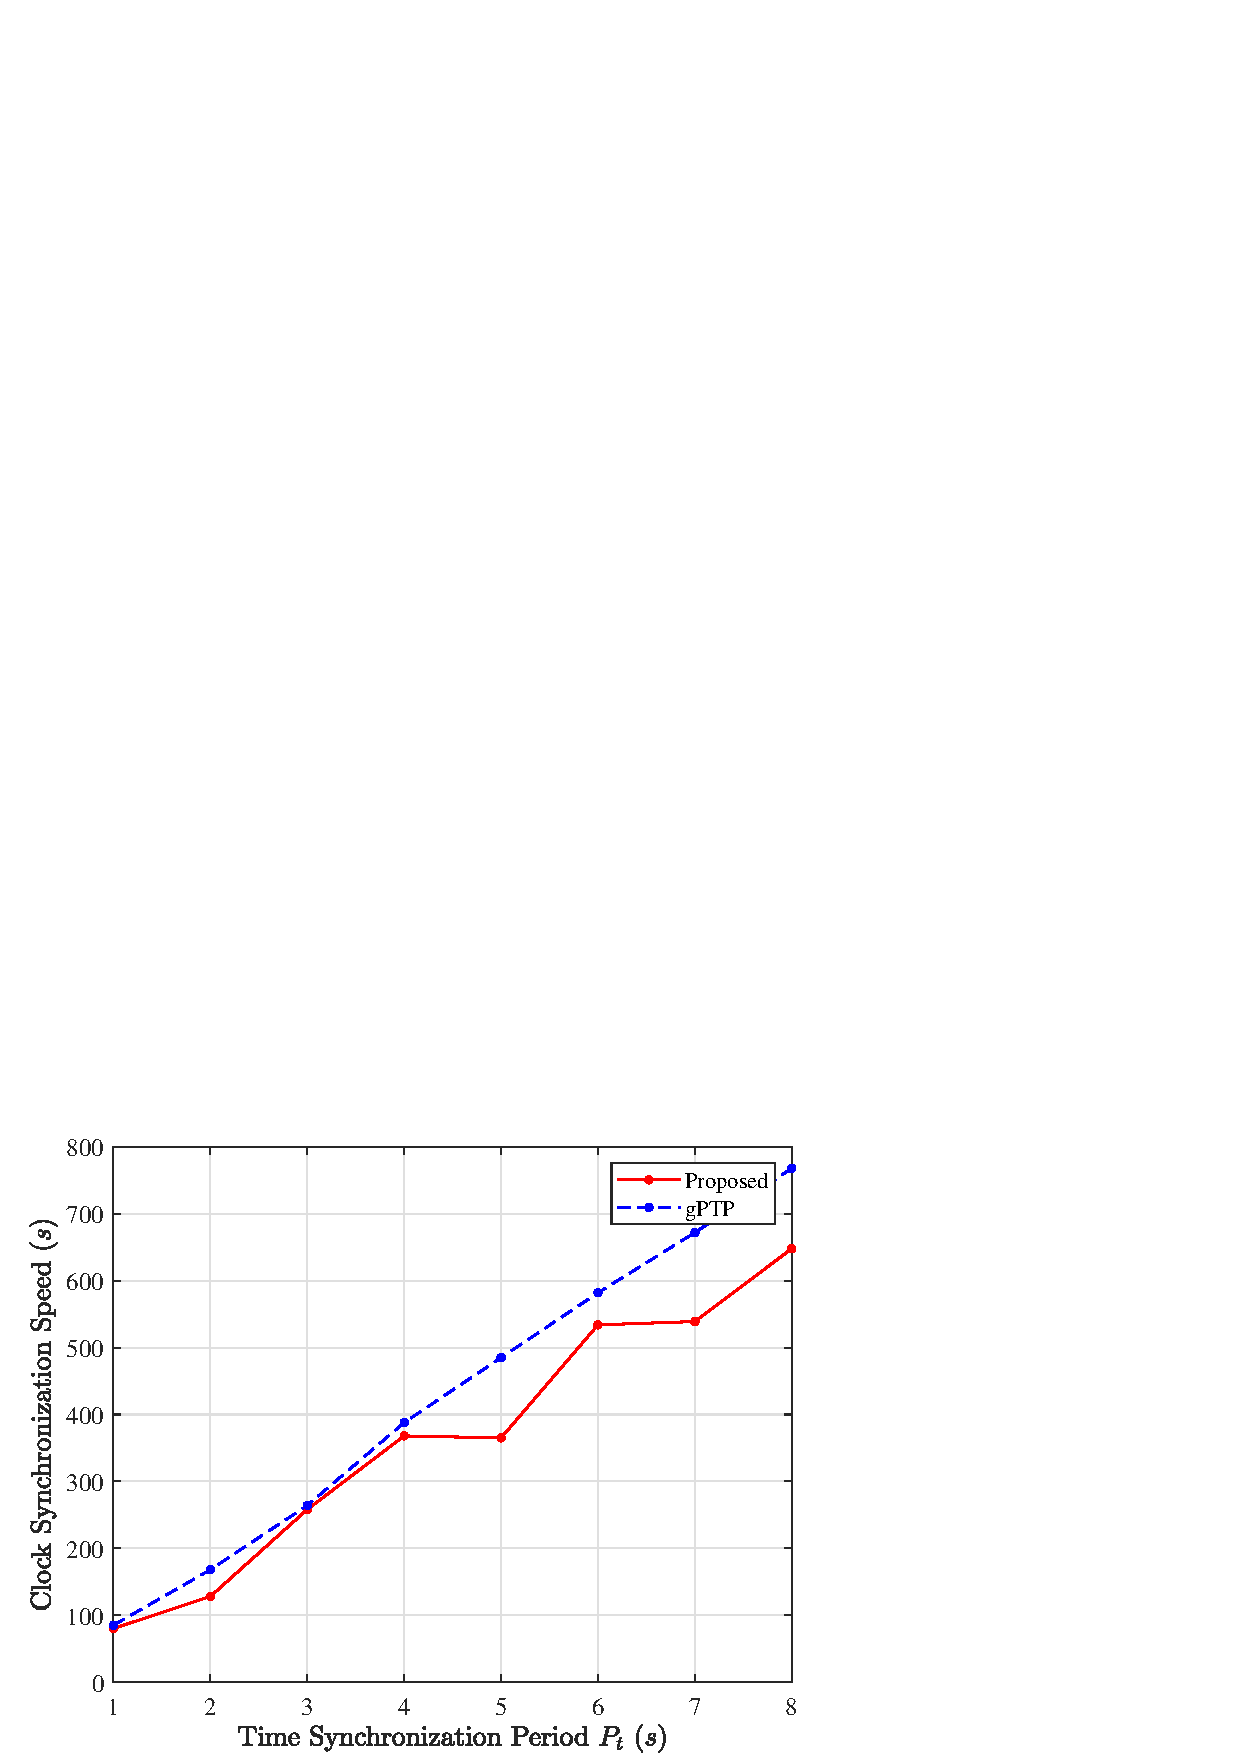
\includegraphics[width=10cm]  {fig8.png}}
	\caption{\label{1} 广播同步}
\end{figure}
\subsection{混合同步架构预览}
混合同步架构是一种专门针对大规模异构网络场景设计的同步方法,在大规模的异构网络协同中有着良好的性能优化,能最小化传输开销,累积误差以及时序误差。如图3-5所示,混合同步架构由有线骨干网络和多个较小无线岛组成,其同步过程主要分为以下三个阶段:
\begin{figure}[htb]
	\center{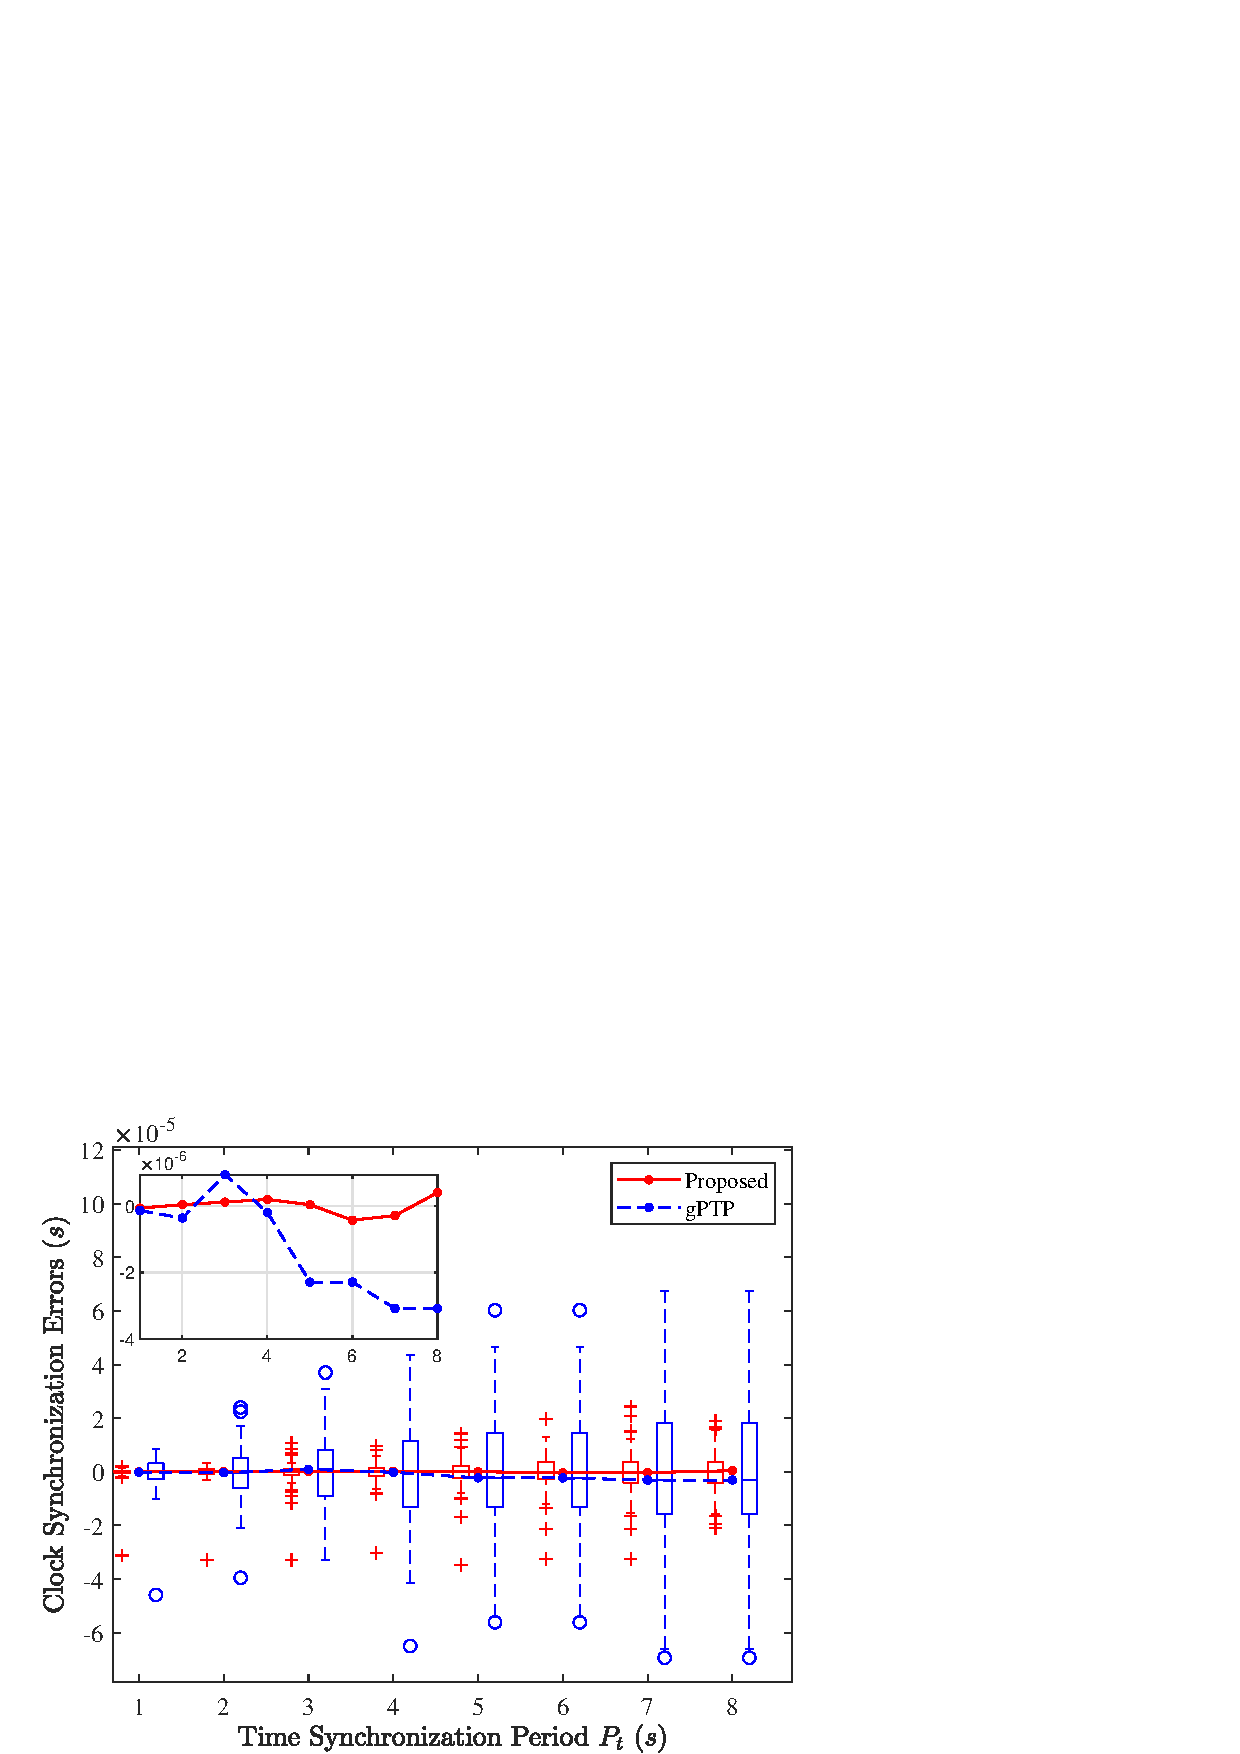
\includegraphics[width=10cm]  {fig7.png}}
	\caption{\label{1} 混合同步架构}
\end{figure}
\begin{itemize}
	\item \textbf{初始化同步:} 在此阶段,有线无线网络先分别进行各自的初始化同步。有线网络通过自带的802.1AS进行同步,无线网络则通过广播方式进行单向同步,其内容包括节点接入,拓扑确认,层级编号以及主从时钟定位。这些参数将被用于确定后续的同步操作,即累积误差补偿和边界补偿。后续阶段的误差补偿都是分层级完成的,没个层级都存在自己的主从时钟配对,配对方式由上文中的参数决定。
	\item \textbf{累积误差补偿:}
	\item \textbf{边界补偿:}
\end{itemize}
\subsection{初始化同步}
\subsubsection{有线部分初始化同步}
有线部分的初始化同步采取gptp同步方案,IEEE 802.1AS 规定了用于 TSN 网络中时间同步的 gPTP。 它定义了传播延迟测量以及频率和时间同步的机制。 gPTP 定义了两种类型的时间感知系统 (TAS),它们是时间感知终端站 (TAE) 和时间感知桥 (TAB)。 TAS 可以是从属实体或主实体。 每个时域只有一个主实体。 此外,在 gPTP 范围内称为大师 (GM) 的主实体充当时间感知网络 (TAN) 内所有从属实体的参考时间源。 TAN 与一个或多个时域相关联。 因此,TAS 可以同时成为不同时域的成员。
时钟偏差补偿方案采用上文中的1588v2协议中的方式进行计算:
\begin{equation*}
	delay = \frac{((t2-t1)+(t4-t3))}{2} 
\end{equation*}
\subsubsection{无线部分初始化同步}
因此混合架构中的无线网络部分可以视为gptp中的一个单独的时域存在,而基站则作为其GM而存在。无线部分的初始化同步则通过广播同步完成,根节点将计数k=0嵌入同步报文广播发送,接收到的节点将计数k进行k+1设定为本地级别并向下一级发送包含k+1的广播同步报文。以此类推。直到所有节点都确定自己的级别,并从上至下依次进行同步。初始同步按照单向同步方案进行,收到广播的时钟根据解包内的时间戳信息和接收时间直接计算传输延时并对本地时钟进行校正。

由于无线部分存在不同的无线通信协议和协同场景,其对于同步精度的要求存在较大差异,例如wifi和wsn网络通常只需要精度达到μs级别即可,因此需要根据组网结构对无线网络中的不同需求创造不同的时域,从而避免通信开销的浪费。对于高精度需求的5G和无线TSN区域,通过成对同步方案进行同步,每次间隔为一个时隙。从时钟会接收到通过中间的若干个来自主时钟的参考时间戳G,并记录下本地时间L。若干组时间戳交换后通过线性回归得到频差和时钟偏差的估计值,并通过下面式子对本地时钟进行修正。
\begin{equation}
	\widehat{L}=L(1+\frac{\widehat{\sigma}}{f_0})-\widehat{o}+[\frac{G_0-L_0}{T_slot}]T_{slot}
\end{equation}
式中的$\sigma$和$o$为线性回归得到的频差和时钟偏差估计值,而公式后半部分则是延时的计算,延时计算最小单位为一个时隙的长度,所以最终测得值应确保为时隙长度的整数倍。时隙长度取决于本章节开头提到的载波间隔长度。

无线部分整体的初始化阶段的同步算法如下:
\begin{algorithm}[ht]  
	\caption{无线网络初始化阶段的时钟同步流程}  
	\begin{algorithmic}[1]
		\REQUIRE GM发送的时间戳, $T_m^1$ and $T_m^2$,$\cdots$, $T_m^n$; 本地节点S记录的时间戳, $T_s^1$ and $T_s^2$,$\cdots$, $T_s^n$; 中央控制系统(CNC)下发的同步精度需求, $prec$;
		\ENSURE 本地的修正时间, $L'$;
		\WHILE {$time \in T_{begin}$}
		\WHILE {$time = nt_slot, n=1,2\ldots $}
		\IF {$prec \geq 500ns$}
		\STATE GM 和无线从节点交换信息, 从节点得到 $T_s^1$ 和 $T_s^2$; 
		\STATE S 计算修正量 $\Delta = [(T_s^1 - T_m^1) - (T_m^2 - T_s^2)]/2$;
		\ELSE  
		\STATE GM 和无线从节点交换信息, 从节点得到 $T_m^1$ and $T_m^2$,$\cdots$, $T_m^n$,通过本地线性回归得到偏差和频率的估计值$\sigma$和$o$	
		\STATE S计算修正量$\widehat{L}=L(1+\frac{\widehat{\sigma}}{f_0})-\widehat{o}+[\frac{G_0-L_0}{T_slot}]T_{slot}$			
		\ENDIF
		\STATE S将层级和修正量参数返回至CNC,等待下一步操作;
		\ENDWHILE
		\ENDWHILE
		%\RETURN $T_{SM}'$.
	\end{algorithmic}
\end{algorithm}

\subsection{累积误差补偿}
在完成初始化同步的阶段之后,混合架构已经完成了有线部分和无线部分的分时域同步,CNC已经确定了网络拓扑结构以及各节点的层级,可以进入累积误差补偿的阶段。

在本阶段中,首先需要在之前标记的高精度同步节点出进行时间戳修正,以确保他们的同步精度。根据2.1的介绍,在同步过程中GM与高精度5G节点之间的传输均被视为透明时钟处理,可以看作单跳累积误差,以此为模型进行修正。在时间戳修正的基础上,需要对时延进一步优化,这将关系到载波间隔的分配和无线传输中的选择性衰弱,从而直接影响到同步精度。

针对不同的精度需求,混合架构依然将采用不同的同步机制,以此来降低总体网络的传输开销。
\subsubsection{时间戳修正}
针对高精度的同步节点,将其与GM之间的部分均视为透明节点,中间部分的同步误差均视为该节点的同步误差,同时参考3.2中得到的与主时钟之间的线性回归频差和偏差估计进行计算。
\begin{figure}[htb]
	\center{\includegraphics[width=10cm]  {fig10.png}}
	\caption{\label{1} 时间戳修正}
\end{figure}
在网络估计时,有线和无线两侧的本地时间可以表示为:
\vspace{-10mm}
\begin{eqnarray}
	\begin{aligned}
		&t_{(\text {wired})}=\left(\alpha_{1}+\sigma_{1}\right) t+\beta_{1}+\delta_{1}\\
		&t_{(\text {wireless })}=\left(\alpha_{2}+\sigma_{2}\right) t+\beta_{2}+\delta_{2}\\
	\end{aligned}
\end{eqnarray}
其中$\alpha_1,\sigma_{1}$为有线侧的频率同步修正估计值与误差,$\alpha_2,\sigma_{2}$为无线侧的频率同步修正估计值与误差,$\beta_1,\delta_{1}$为有线侧的时偏同步修正估计值与误差,$\beta_2,\delta_{2}$为无线侧的时偏同步修正估计值与误差,t代表参考时钟的时间。由于两侧的时偏和频率估计存在精度差距,因此有线无线在进行时间戳交换的时钟同步时,会造成边界同步误差。\\
对于左侧有线主时钟而言,发送的sync报文包含$t_1$时刻的时间戳,此时对应的参考时间应为$t=\frac{t_{1}-\beta_{1}-\delta_{1}}{\alpha_{1}+\sigma_{1}}$,当此报文到达无线侧从时钟时,从时钟接收并记录时间戳$t_2$,该时间戳的值应为$t_{2}=\left(\frac{t_{1}-\beta_{1}-\delta_{1}}{\alpha_{1}+\sigma_{1}}+\text { delay }\right)\left(\alpha_{2}+\sigma_{2}\right)+\beta_{2}+\delta_{2}$,其中delay即为从有线侧到无线侧的传输时间。\\
同理,当无线侧向有线侧发送同步请求需求的Delay\_req报文时,报文内的时间戳$t_3$对应的参考时间应为$t=\frac{t_{3}-\beta_{2}-\delta_{2}}{\alpha_{2}+\sigma_{2}}$,当此报文到达有线侧从时钟时,从时钟接收并记录时间戳$t_4$,该时间戳的值应为$t_{4}=\left(\frac{t_{3}-\beta_{2}-\delta_{2}}{\alpha_{2}+\sigma_{2}}+\text { delay }\right)\left(\alpha_{1}+\sigma_{1}\right)+\beta_{1}+\delta_{1}$,其中delay即为从无线侧到有线侧的传输时间。\\
实际应用中,在进行时钟同步时,对于传输时延通常采用对称化处理,即$2 \text { delay }=t_{2}-t_{1}+t_{4}-t_{3}$,由于上述提到的两侧精度的不同,实际上的传输时延应该为$2 \text { delay }=m\left(t_{2}-t_{1}+t_{4}-t_{3}\right)-(m-1 / m)\left(\beta_{1}+\delta_{1}\right)+(m-1 / m)\left(\beta_{2}+\delta_{2}\right)$,其中$m=\frac{\alpha_{2}+\sigma_{2}}{\alpha_{1}+\sigma_{1}}$,由于有线部分同步误差$\ll$无线部分的同步误差,因此式中的$(m-1 / m)\left(\beta_{1}+\delta_{1}\right)$可忽略不计,因此对于传输时延的计算公式可以化简为$2 \text { delay }=m\left(t_{2}-t_{1}+t_{4}-t_{3}\right)-(m-1 / m)\left(\beta_{2}+\delta_{2}\right)$,采用此公式修正传输延时的计算结果,可以在不需要反复多次交换时间戳的情况下,有效提升时间同步精度,增加时钟同步效率。
\begin{eqnarray}
	&t_{1}=\left(\alpha_{1}+\sigma_{1}\right) t+\beta_{1}+\delta_{1}\\
	&t=\frac{t_{1}-\beta_{1}-\delta_{1}}{\alpha_{1}+\sigma_{1}}\\
	&t_{2}=\left(\frac{t_{1}-\beta_{1}-\delta_{1}}{\alpha_{1}+\sigma_{1}}+\text { delay }\right)\left(\alpha_{2}+\sigma_{2}\right)+\beta_{2}+\delta_{2}\\
	&t=\frac{t_{3}-\beta_{2}-\delta_{2}}{\alpha_{2}+\sigma_{2}}\\
	&t_{4}=\left(\frac{t_{3}-\beta_{2}-\delta_{2}}{\alpha_{2}+\sigma_{2}}+\text { delay }\right)\left(\alpha_{1}+\sigma_{1}\right)+\beta_{1}+\delta_{1}
\end{eqnarray}
\begin{eqnarray}
	\begin{gathered}
		m=\frac{\alpha_{2}+\sigma_{2}}{\alpha_{1}+\sigma_{1}}\\
		2 \text { delay }=t_{2}-t_{1}+t_{4}-t_{3} \\
		2 \text { delay }=m\left(t_{2}-t_{1}+t_{4}-t_{3}\right)-(m-1 / m)\left(\beta_{1}+\delta_{1}\right)+(m-1 / m)\left(\beta_{2}+\delta_{2}\right) \\
		2 \text { delay }=m\left(t_{2}-t_{1}+t_{4}-t_{3}\right)-(m-1 / m)\left(\beta_{2}+\delta_{2}\right)
	\end{gathered}
\end{eqnarray}
\subsubsection{传输延迟优化}
在进行时间戳修正后,时钟同步对于传输延迟的计算精度提高了,但是由于无线有线传输的不确定性,当传输延迟较大时,计算的误差也会增加,从而增加累积误差。同时,无线内部的时钟同步公式$\widehat{L}=L(1+\frac{\widehat{\sigma}}{f_0})-\widehat{o}+[\frac{G_0-L_0}{T_slot}]T_{slot}$中,影响时间戳修正精度的关键因素即为时隙$T_{slot}$的大小,在5G传输中,时隙的大小与传输延迟也息息相关。综上,累积误差造成的影响取决于同步过程中时隙的大小,时隙决定了同步精度的精度上限,当节点数目增多时,同步延迟增大,时隙长度对累积误差的影响就更明显。\\
由于研究对象为以5G为载体的无线TSN网络,5G网络帧结构如下图所示:
\begin{figure}[htb]
	\center{\includegraphics[width=10cm]  {fig11.png}}
	\caption{\label{1} 5G帧结构}
\end{figure}
5G中无线帧和子帧的长度是相同的,无线帧为10ms,子帧长度为1ms
5G中一个时隙包含的ofdm符号数量为14,不同的载波间隔下每个子帧包含的时隙数量不同
ssb(时钟同步报文)固定占有4个ofdm符号,所以不同的子载波间隔下ssb的持续时间和周期不同,5G子载波间隔是可调整的,例如,在实际应用中,5G协议有给出不同应用场景下推荐的子载波间隔参数集。
\begin{figure}[htb]
	\center{\includegraphics[width=10cm]  {fig12.png}}
	\caption{\label{1} 常见载波分配参数集}
\end{figure}
然而上述所给出的应用案例中,即使是时隙最小的情况,所对应的传输延迟也会达到ms级别,并不能达到无线TSN和有线TSN的精度需求,因此需要进一步进行优化。\\
由于5G网络子载波间隔的可分配这一特性,通过增大子载波间隔来减少子载波数量,减少ofdm的符号长度,从而降低时延,减少累积误差。
在大致的传输环境一定的情况下,相干带宽是相同的,子载波间隔(即子载波带宽)越大,子载波数量越少,每个子载波的带宽越大,产生频率选择性衰弱的可能性越高(信号带宽大于相干性带宽时才会发生)。 因此在仿真时需要先满足时延需求再利用均衡器进行补偿,保证同步精度。
\subsubsection{校验更新}
在完成累积误差补偿后,混合架构需要对网络参数进行更新。首先是对于网络拓扑的校验更新。原有的网络节点在后续的网络拓展中不需要进行任何更新,因为网络拓展没有打破他们原有的主从关系链。原有的网络拓扑同步规则将会保留,以节省传输资源,因此需要更新的就是新增的网络节点的本地校验,由于新增的无线终端节点分布的不确定性,如果直接取与有线主时钟的主从关系,势必要从其他的原有节点中取得原有的网络参数值,从而带来更多的跨机传输开销,因此选择将其作为一个新增的局域网络,和就近的无线节点进行同步,即将该对接的无线节点视为之前混合架构中的高精度有线主时钟,并采用之前的同步优化规则对新增节点进行同步,这样可以有效节省计算开销,并且由于原有无线节点已经进行过累积误差优化,这样所带来的误差在可接受的范围内。\\
接下来进行的全局校验的生成。由于原有拓扑网络节点的离线或故障,或者当同步精度漂移较大时,则需要对原有架构参数进行更新,重新计算频偏和时偏的估计值。每次全局校验更新都需要从其他节点中获取数据,会产生极大的传输开销,而且这部分的更新校验是不可避免的。\\
为了降低全局校验更新带来的跨节点传输开销,混合架构可以在结构内优先进行数据的计算,生成一些中间的结果,最后只将这些中间结果传输至出现同步问题需要进行全局校验的节点。这些中间结果能够代替原始数据完成校验的运算,保证了校验更新的正确性,并且相较于原始数据,中间结果能够将多个数据块运算成一个数据块,节省了跨节点传输的开销。
更新校验的整体算法如下:
\begin{algorithm}[ht]  
	\caption{无线网络初始化阶段的新增更新校验流程}  
	\begin{algorithmic}[1]
		\REQUIRE mode:新增校验or全局校验,新增GM的层级,$l_{新增GM}$, 新增GM发送的时间戳,$T_m^1$ and $T_m^2$,$\cdots$, $T_m^n$; 新增节点S记录的时间戳, $T_s^1$ and $T_s^2$,$\cdots$, $T_s^n$; 中央控制系统(CNC)下发的同步精度需求, $prec$;
		\ENSURE 本地的修正时间, $L'$;
		\IF{mode=新增校验}
		\STATE 接入5G网络后,通过基站找到距离最近的原无线网络节点,将其设定为新增GM
		\WHILE {$time \in T_{update}$}
		\WHILE {$time = nt_{slot}, n=1,2\ldots $}
		\IF {$prec \geq 500ns$}
		\STATE 新增GM 和无线从节点交换信息, 从节点得到 $T_s^1$ 和 $T_s^2$; 
		\STATE S 计算修正量 $\Delta = [(T_s^1 - T_m^1) - (T_m^2 - T_s^2)]/2$;
		\STATE S 计算层级$l=l_{新增GM}+k$
		\ELSE  
		\STATE 新增GM 和无线从节点交换信息, 从节点得到 $T_m^1$ and $T_m^2$,$\cdots$, $T_m^n$,通过本地线性回归得到偏差和频率的估计值$\sigma$和$o$	
		\STATE S计算修正量$\widehat{L}=L(1+\frac{\widehat{\sigma}}{f_0})-\widehat{o}+[\frac{G_0-L_0}{T_slot}]T_{slot}$			
		\ENDIF
		\STATE S将层级和修正量参数返回至CNC,等待下一步操作;
		\ENDWHILE
		\ENDWHILE
		\ENDIF
		%\RETURN $T_{SM}'$.
	\end{algorithmic}
\end{algorithm}




\subsection{本章小结}
本章介绍了本文所提出的混合同步架构,并详细介绍了混合同步架构的三个同步阶段,包括计算频偏和时偏估计值,达成初步时钟一致的初始化同步阶段,针对异构网络中的累积误差进行的补偿阶段,以及最后完成校验更新保证同步可靠性的校验更新阶段。
第二章中提到的异构网络同步需求,混合同步架构完美地满足了这些需求。
\begin{itemize}
	\item 混合架构达到了高精度的无线TSN网络同步需求。
	\item 混合架构实现了最小网络传输开销,因为逐层同步只会从原有节点至新增节点。
	\item 混合架构解决了异构网络传输时延不一致的问题。
	\item 混合架构保证了最小的更新校验量,因为校验链被尽量地保留,从而减少了需要更新的校验块个数。
\end{itemize}

\newpage
\fancyhead[LH]{上海交通大学学位论文}
\fancyhead[RH]{第四章\quad全文总结}
\section{仿真实验}

\section{全文总结}

\subsection{主要结论}
本文主要……

\subsection{研究展望}
更深入的研究……
\begin{table}[!htbp]
	\centering
	\caption{高频感应加热的基本参数}
	\begin{tabular}{|c| c|c|c|}
		\hline
		感应频率 &感应发生器功率 & 工件移动速度  &感应圈与零件间隙\\
		(KHz)&($\% \times$80Kw) &(mm/min)  &(mm)\\
		\hline
		250 &88 &5900 &1.65\\
		\hline
		250 &88 &5900 &1.65\\
		\hline
		250 &88 &5900 &1.65\\
		\hline
		250 &88 &5900 &1.65\\
		\hline
		250 &88 &5900 &1.65\\
		\hline
		250 &88 &5900 &1.65\\
		\hline
		250 &88 &5900 &1.65\\
		\hline
		250 &88 &5900 &1.65\\
		\hline
	\end{tabular}
\end{table}

\begin{table}
	\centering
	\captionsetup{singlelinecheck=off}
	\caption*{续表} %取消编号
	\begin{tabular}{|c| c|c|c|}
		\hline
		感应频率 &感应发生器功率 & 工件移动速度  &感应圈与零件间隙\\
		(KHz)&($\% \times$80Kw) &(mm/min)  &(mm)\\
		\hline
		250 &88 &5900 &1.65\\
		\hline
		250 &88 &5900 &1.65\\
		\hline
	\end{tabular}
\end{table}
%表格太大需要转页时,需要在续表上方注明“续表”,表头也应重复排出。

\newpage
\fancyhead[LH]{上海交通大学学位论文}
\fancyhead[RH]{参考文献}

\addcontentsline{toc}{section}{参\quad考\quad文\quad献}
\renewcommand\refname{参\quad考\quad文\quad献}
\begin{thebibliography}{1}
\bibitem{1} 杨瑞林, 李力军. 新型低合金高强韧性耐磨钢的研究. 钢铁. 1999(7):41~45.
\bibitem{2}  Schinstock, D.E., Cuttino, J.F. Real time kinematic solutions of a non-contacting, three dimensional metrology frame[J]. Precision Engineering. 2000, 24(1):70-76. 
\bibitem{3} 温诗铸. 摩擦学原理. 北京:清华大学出版社. 1990:296-300.
\bibitem{4} 贾名字. 工程硕士论文撰写规范[硕士论文].上海:上海交通大学. 2000.
\bibitem{5} 姜锡洲.一种温热外敷药制备方案[P].中国专利:881056078,1983-08-12.
\bibitem{6}]GB/T16159—1996,汉语拼音正词法基本规则[S].北京:中国标准出版社,1996.
\end{thebibliography}

\newpage
\fancyhead[LH]{上海交通大学学位论文}
\fancyhead[RH]{附录1}

\addcontentsline{toc}{section}{附录}
\section*{符号与标记(附录1)}

\newpage
\fancyhead[LH]{上海交通大学学位论文}
\fancyhead[RH]{学术论文和科研成果目录}

\addcontentsline{toc}{section}{攻读学位期间学术论文和科研成果目录}
\section*{攻读学位期间学术论文和科研成果目录}

[1] 张三,李四. …… (已录用)

\newpage
\fancyhead[LH]{上海交通大学学位论文}
\fancyhead[RH]{致\qquad谢}

\addcontentsline{toc}{section}{致\qquad谢}
\section*{致\qquad谢}

\hspace{8mm}致谢主要感谢导师和对论文工作有直接贡献和帮助的人士和单位。致谢言语应谦虚诚恳,实事求是。





\end{document} 